\newpage
\section*{Technical}
\label{sec:technical}
This section provides a high-level overview of my current application's
architecture and methodologies. It highlights areas where collaboration with
Decision Brain can enhance the project's success and offers insights that may
benefit Decision Brain's own practices.

\subsection*{Architecture of the Scheduling System}
I have spent a significant part of my Ph.D. program refining and testing different architectures to enable
meta-heuristics to coordinator state in real-time. The latest version is shown in figure~\ref{fig:ordinator:architecture}.

\begin{figure}[H]
	\centering
	\usetikzlibrary {positioning}

\definecolor{red}{HTML}{8A3F3A}
\definecolor{yellow}{HTML}{E0BB3C}
\definecolor{blue}{HTML}{4569E0}
\definecolor{green}{HTML}{17E561}
\definecolor{other}{HTML}{6A939E}

% DTU Colors
\definecolor{dtu-corporate-red}{HTML}{990000}
\definecolor{dtu-white}{HTML}{ffffff}
\definecolor{dtu-black}{HTML}{000000}
\definecolor{dtu-blue}{HTML}{2F3EEA}
\definecolor{dtu-bright-green}{HTML}{1FD082}
\definecolor{dtu-navy-blue}{HTML}{030F4F}
\definecolor{dtu-yellow}{HTML}{F6D04D}
\definecolor{dtu-orange}{HTML}{FC7634}
\definecolor{dtu-pink}{HTML}{F7BBB1}
\definecolor{dtu-grey}{HTML}{DADADA}
\definecolor{dtu-red}{HTML}{E83F48}
\definecolor{dtu-green}{HTML}{008835}
\definecolor{dtu-purple}{HTML}{79238E}


\newcommand{\ModelColor}{dtu-red}
\newcommand{\UserInterfaceColor}{dtu-yellow}
\newcommand{\PersistenceColor}{dtu-blue}
\newcommand{\PointerSwapColor}{dtu-green}
\newcommand{\OrchestratorColor}{dtu-bright-green}

\newcommand{\basisinput}{4cm}  % Default value if not set by /graph/basis

\pgfkeys{
	/graph/.is family, /graph,
	default/.style = {
		show_shared_pointer = false,
		show_orchestrator = false,
		show_persistence = false,
		show_user_interface = false,
		basisinput/.estore in = \basisinput,
	},
	show_shared_pointer/.estore in = \ShowSharedSolutionCommunication,
	show_orchestrator/.estore in = \ShowOrchestratorCommunication,
	show_persistence/.estore in = \ShowPersistenceCommunication,
	show_user_interface/.estore in = \ShowUserInterfaceCommunication,
	basisinput/.estore in = \basisinput,
}

\newlength{\basis}
\tikzset{
  basis/.code={\setlength{\basis}{\basisinput}}, % TikZ assignment code
  basis/.default=3cm,                   % Provide a default (\b@sis is undefined/unassigned)
  basis,                                % Set initial Value (\b@sis is defined/assigned)
}

\newcommand{\drawOrdinatorArchitecture}[1]{
	\pgfkeys{/graph, default, #1}
	\setlength{\basis}{\basisinput}
	\begin{tikzpicture}[scale=0.75, line width=0.05\basis]

		\ifthenelse{\equal{\ShowOrchestratorCommunication}{true}}{
			\draw[color=other,-, ultra thick] (Strategic) -- (Orchestrator);
			\draw[color=other,-, ultra thick] (Tactical) -- (Orchestrator);
			\draw[color=other,-, ultra thick] (Supervisor) -- (Orchestrator);
			\draw[color=other,-, ultra thick] (Operational_1) -- (Orchestrator);
			\draw[color=other,-, ultra thick] (Operational_2) -- (Orchestrator);
			\draw[color=other,-, ultra thick] (Operational_3) -- (Orchestrator);
		}{}
		% \draw[help lines] (0\basis, 0\basis) grid (10\basis, 8\basis);
		\draw (5\basis,4\basis) node[minimum height=5\basis,minimum width=7.0\basis,rounded corners=0.1\basis] {};

	    \draw[draw=black] (4.125\basis,4.0\basis) node[opacity=0.5, minimum height=3.5\basis,minimum width=6.25\basis,rounded corners=0.1\basis,fill=\PointerSwapColor] {} ;
	    \draw (2.5\basis,5.5\basis) node[minimum height=1\basis,minimum width=1\basis,fill=\ModelColor,rounded corners=0.1\basis] (Strategic) {Stra};
	    \draw (5.0\basis,4.0\basis) node[minimum height=1\basis,minimum width=1\basis,fill=\ModelColor,rounded corners=0.1\basis] (Supervisor) {Sup};
		\draw (7.5\basis,5.5\basis) node[minimum height=1\basis,minimum width=1\basis,fill=\ModelColor,rounded corners=0.1\basis] (Tactical) {Tac};

		\draw (2.5\basis,2.5\basis) node[minimum height=1\basis,minimum width=1\basis,fill=\ModelColor,rounded corners=0.1\basis] (Operational_1) {$O_{1}$};
		\draw (5.0\basis,2.5\basis) node[minimum height=1\basis,minimum width=1\basis,fill=\ModelColor,rounded corners=0.1\basis] (Operational_2) {$O_{2}$};
		\draw (7.5\basis,2.5\basis) node[minimum height=1\basis,minimum width=1\basis,fill=\ModelColor,rounded corners=0.1\basis,rounded corners=0.1\basis] (Operational_3) {$O_{3}$};
	
		\draw (Strategic) edge (Tactical);
		\draw (Strategic) edge (Tactical);
		\draw (5\basis,5.5\basis) edge (Supervisor);
		\draw (Supervisor) -- (2.5\basis,4.0\basis) -- (Operational_1);
		\draw (Supervisor) edge (Operational_2);
		\draw (Supervisor) -- (7.5\basis,4.0\basis) -- (Operational_3);
		\draw (5.0\basis,0.5\basis)   node[minimum height=1\basis,minimum width=5.0\basis,                fill=\PersistenceColor,rounded corners=0.1\basis] {persistence};
		\draw (5.0\basis,7.5\basis)   node[minimum height=1\basis,minimum width=5.0\basis,                fill=\OrchestratorColor,rounded corners=0.1\basis] (Orchestrator) {Orchestrator};
		\draw (0.5\basis,4.0\basis)   node[rotate=90, minimum height=1.0\basis, minimum width=3.5\basis,  fill=\PointerSwapColor,rounded corners=0.1\basis] {decision variables};
		\draw (9.5\basis,5.75\basis)  node[rotate=90, minimum height=1.0\basis, minimum width=1.0\basis,  fill=\UserInterfaceColor,rounded corners=0.1\basis] {UI};
		\draw (9.5\basis,4.0\basis)   node[rotate=90, minimum height=1.0\basis, minimum width=1.0\basis,  fill=\UserInterfaceColor,rounded corners=0.1\basis] {UI};
		\draw (9.5\basis,2.25\basis)  node[rotate=90, minimum height=1.0\basis, minimum width=1.0\basis,  fill=\UserInterfaceColor,rounded corners=0.1\basis] {UI};

		% Legend
		\begin{scope}[shift={(11.0\basis,5.7\basis)}]
			\node at (-0.25\basis,1\basis) [right] {};
			\draw[color=\OrchestratorColor,fill,rounded corners=0.1\basis] (0\basis,0.0\basis)   rectangle (0.5\basis, 0.5\basis);
			\node[anchor=west] at (0.5\basis, 0.25\basis) { Managing metaheuristic lifetimes };
			\draw[color=\PointerSwapColor,fill,rounded corners=0.1\basis] (0\basis,-1.0\basis)   rectangle(0.5\basis, -0.5\basis); 
			\node[anchor=west] at (0.5\basis, -0.75\basis) { Solution sharing (Atomic pointer swaps) };
			\draw[color=\ModelColor,fill,rounded corners=0.1\basis] (0\basis,-2.0\basis)         rectangle(0.5\basis, -1.5\basis); 
			\node[anchor=west] at (0.5\basis, -1.75\basis) { Metaheurics (Mathematical Models) };
			\draw[color=\PersistenceColor,fill,rounded corners=0.1\basis] (0\basis,-3.0\basis)   rectangle(0.5\basis, -2.5\basis); 
			\node[anchor=west] at (0.5\basis, -2.75\basis) { Data storage (Memory locks)};
			\draw[color=\UserInterfaceColor,fill,rounded corners=0.1\basis] (0\basis,-4.0\basis) rectangle(0.5\basis, -3.5\basis); 
			\node[anchor=west] at (0.5\basis, -3.75\basis) { Message passing (Memory channels) };

		\end{scope}
		\ifthenelse{\equal{\ShowSharedSolutionCommunication}{true}}{
			\draw[->, thick] (Strategic) -- (Orchestrator);
		}{}
		\ifthenelse{\equal{\ShowUserInterfaceCommunication}{true}}{
			\draw[->, thick] (Strategic) -- (Orchestrator);
		}{}
		\ifthenelse{\equal{\ShowPersistenceCommunication}{true}}{
			\draw[->, thick] (Strategic) -- (Orchestrator);
		}{}
		

	\end{tikzpicture}
}


	\drawOrdinatorArchitecture{basisinput=1cm}

	\caption{
		High level architecture of the scheduling system. Persistence stores
		all data, whether from SAP, user input, or other systems; the Orchestrator manages the lifetimes of the 
		metaheuristics; the metaheuristics does the actual optimization;
		the decision variable are all stored together and are shared among all optimizating meta-heuristics, 
		each algorithm can write to its own state but only read the state of its neighbors; the UI components
		each communicate with the algorithms that correspond to the individual stakeholder, meaning that the 
		models also specify what each stakeholder is allowed to modify.
	}
	\label{fig:ordinator:architecture}
\end{figure}

\textbf{Key Lessons:}
\begin{itemize}
	\item Message passing between metaheuristics are unworkable, e.g. a microservice architecture is difficult approach. A usable scheduling
	      system needs to be implemented on a single CPU with multi-threading, "normal" best practice for horizontal scaling is difficult as 
		  state changes quickly in metaheuristics. 
	\item Optimization problems are difficult due to large and complex solution spaces. Allowing models/meta-heuristics
		  to use each others solutions as parameters allows you to keep solution spaces smaller while preserving the 
		  ability to model the larger system (sacrificing global optimization which is usually meaningless in practice).
	\item The operational setting is more complex than it appears and changes faster than you think. Developing large integrated models 
		  is difficult as model changes become both more difficult and frequent the larger the model gets. This tends to make
		  such scheduling systems fragile.
\end{itemize}

The key feature that this architecture enable is that we can move away from hierarchical approaches and 
instead model each stakeholder individually with the responsibilities that exactly that person is responsible 
for. In figure~\ref{fig:model-setup:hexagon} we see that the system can initialize many instances of each metaheuristic, each corresponding to a stakeholder. 

\begin{figure}[H]
	\usetikzlibrary {positioning}
\newcommand{\drawHexagon}[6][draw=black]{
	\draw[#1, fill=#4] (#2,#3) ++(30:#6) -- ++(90:#6) -- ++(150:#6) -- ++(210:#6) -- ++(270:#6) -- ++(330:#6) -- cycle;
	\node[align=center] at (#2,#3+2) {#5};
}

\newif\ifpersistencelayer
\newif\ifatomicpointerswaplayer
\newif\ifmetaheuristicslayer
\newif\ifuserinterfacelayer
\newif\iforchestratorlayer
\newif\ifsimplifiedlayer

\pgfkeys{
	/hexagon/.is family, /hexagon,
	default/.style = {
		persistence=false,
		atomicpointerswap=false,
		metaheuristics=false,
		orchestrator=false,
		userinterface=false,
		simplified=false,
	},
	persistence/.is if=persistencelayer,
	atomicpointerswap/.is if=atomicpointerswaplayer,
	metaheuristics/.is if=metaheuristicslayer,
	orchestrator/.is if=orchestratorlayer,
	userinterface/.is if=userinterfacelayer,
	simplified/.is if=simplifiedlayer,
}
\newcommand{\drawModelSetupHexagon}[1][]{
	\pgfkeys{/hexagon, default, #1}

	\begin{tikzpicture}[font=\footnotesize, scale=0.5, line width=1.05]
	

	\ifpersistencelayer
		\drawHexagon[draw=none]{ 2                      }{ 2}{dtu-blue}{}{2}
		\drawHexagon[draw=none]{{6 - 2 * (2 - sqrt(3)) }}{ 2}{dtu-blue}{}{2}
		\drawHexagon[draw=none]{{4 - 1 * (2 - sqrt(3)) }}{-1}{dtu-blue}{Persistence}{2}
		\drawHexagon[draw=none]{{0 + 1 * (2 - sqrt(3)) }}{-1}{dtu-blue}{}{2}
		\drawHexagon[draw=none]{{8 - 3 * (2 - sqrt(3)) }}{-1}{dtu-blue}{}{2}

		\drawHexagon[draw=none]{{2 - 0 * (2 - sqrt(3)) }}{-4}{dtu-blue}{}{2}
		\drawHexagon[draw=none]{{6 - 2 * (2 - sqrt(3)) }}{-4}{dtu-blue}{}{2}

		\drawHexagon[draw=none]{{10 - 4 * (2 - sqrt(3)) }}{-4}{dtu-blue}{}{2}
		\drawHexagon[draw=none]{{-2 + 2 * (2 - sqrt(3)) }}{-4}{dtu-blue}{}{2}

		\drawHexagon[draw=none]{{12 - 5 * (2 - sqrt(3)) }}{-1}{dtu-blue}{}{2}
		\drawHexagon[draw=none]{{-4 + 3 * (2 - sqrt(3)) }}{-1}{dtu-blue}{}{2}
		% Legend for each layer
		\drawHexagon{{14.0  }}{+3.0}{dtu-blue}{}{0.75}
		\node[align=right, anchor=west] at ({15.0}, +3.75) {Persistence};
		\drawHexagon{{14.0  }}{+1.5}{dtu-white}{}{0.75}
		\node[align=right, anchor=west] at ({15.0}, +2.25) {Atomic Pointer};
		\drawHexagon{{14.0  }}{+0.0}{dtu-white}{}{0.75}
		\node[align=right, anchor=west] at ({15.0}, +0.75) {Metaheuristics};
		\drawHexagon{{14.0  }}{-1.5}{dtu-white}{}{0.75}
		\node[align=right, anchor=west] at ({15.0}, -0.75) {Orchestration};
		\drawHexagon{{14.0  }}{-3.0}{dtu-white}{}{0.75}
		\node[align=right, anchor=west] at ({15.0}, -2.25) {User interfaces};
	\fi


	\ifatomicpointerswaplayer
		\drawHexagon[]{ 2                      }{ 2}{dtu-green}{Shared\\solution\\pointer}{2}
		\drawHexagon[]{{6 - 2 * (2 - sqrt(3)) }}{ 2}{dtu-green}{Shared\\solution\\pointer}{2}
		\drawHexagon[]{{4 - 1 * (2 - sqrt(3)) }}{-1}{dtu-green}{Shared\\solution\\pointer}{2}
		\drawHexagon[]{{0 + 1 * (2 - sqrt(3)) }}{-1}{dtu-green}{Shared\\solution\\pointer}{2}
		\drawHexagon[]{{8 - 3 * (2 - sqrt(3)) }}{-1}{dtu-green}{Shared\\solution\\pointer}{2}

		\drawHexagon[]{{2 - 0 * (2 - sqrt(3)) }}{-4}{dtu-green}{Shared\\solution\\pointer}{2}
		\drawHexagon[]{{6 - 2 * (2 - sqrt(3)) }}{-4}{dtu-green}{Shared\\solution\\pointer}{2}

		\drawHexagon[]{{10 - 4 * (2 - sqrt(3)) }}{-4}{dtu-green}{Shared\\solution\\pointer}{2}
		\drawHexagon[]{{-2 + 2 * (2 - sqrt(3)) }}{-4}{dtu-green}{Shared\\solution\\pointer}{2}

		\drawHexagon[]{{12 - 5 * (2 - sqrt(3)) }}{-1}{dtu-green}{Shared\\solution\\pointer}{2}
		\drawHexagon[]{{-4 + 3 * (2 - sqrt(3)) }}{-1}{dtu-green}{Shared\\solution\\pointer}{2}
		% Legend for each layer
		\drawHexagon{{14.0  }}{+3.0}{dtu-white}{}{0.75}
		\node[align=right, anchor=west] at ({15.0}, +3.75) {Persistence};
		\drawHexagon{{14.0  }}{+1.5}{dtu-green}{}{0.75}
		\node[align=right, anchor=west] at ({15.0}, +2.25) {Atomic Pointer};
		\drawHexagon{{14.0  }}{+0.0}{dtu-white}{}{0.75}
		\node[align=right, anchor=west] at ({15.0}, +0.75) {Metaheuristics};
		\drawHexagon{{14.0  }}{-1.5}{dtu-white}{}{0.75}
		\node[align=right, anchor=west] at ({15.0}, -0.75) {Orchestration};
		\drawHexagon{{14.0  }}{-3.0}{dtu-white}{}{0.75}
		\node[align=right, anchor=west] at ({15.0}, -2.25) {User interfaces};
	\fi

	\ifsimplifiedlayer

		\node[align=right, anchor=west] at ({-5.5}, +3.75) {};
		\drawHexagon{{+2 + 0 * (2 - sqrt(3)) }}{ 2}{dtu-green}{Scheduler}{2}
		\drawHexagon{{+4 - 1 * (2 - sqrt(3)) }}{-1}{dtu-red}{Supervisor}{2}
		\drawHexagon{{+0 + 1 * (2 - sqrt(3)) }}{-1}{dtu-red}{Supervisor}{2}
		\drawHexagon{{+2 - 0 * (2 - sqrt(3)) }}{-4}{dtu-corporate-red}{Technician}{2}
		\drawHexagon{{+6 - 2 * (2 - sqrt(3)) }}{-4}{dtu-corporate-red}{Technician}{2}
		\drawHexagon{{-2 + 2 * (2 - sqrt(3)) }}{-4}{dtu-corporate-red}{Technician}{2}
		\drawHexagon{{+8 - 3 * (2 - sqrt(3)) }}{-1}{dtu-corporate-red}{Technician}{2}
		\drawHexagon{{-4 + 3 * (2 - sqrt(3)) }}{-1}{dtu-corporate-red}{Technician}{2}

		% Scheduler
		\draw[thin, fill=dtu-yellow] (2, 5) circle (0.35);
		\draw[thin, fill=dtu-purple] (2, 3) circle (0.35);
		% Supervisor 1
		\draw[thin, fill=dtu-yellow] ({+4 - 1 * (2 - sqrt(3)) }, 02) circle (0.35);
		\draw[thin, fill=dtu-purple] ({+4 - 1 * (2 - sqrt(3)) }, -0) circle (0.35);
		% Supervisor 2
		\draw[thin, fill=dtu-yellow] ({+0 + 1 * (2 - sqrt(3)) }, 02) circle (0.35);
		\draw[thin, fill=dtu-purple] ({+0 + 1 * (2 - sqrt(3)) }, -0) circle (0.35);
		% Technician 1
		\draw[thin, fill=dtu-yellow] ({+2 - 0 * (2 - sqrt(3)) }, -1) circle (0.35);
		\draw[thin, fill=dtu-purple] ({+2 - 0 * (2 - sqrt(3)) }, -3) circle (0.35);
		% Technician 2
		\draw[thin, fill=dtu-yellow] ({+6 - 2 * (2 - sqrt(3)) }, -1) circle (0.35);
		\draw[thin, fill=dtu-purple] ({+6 - 2 * (2 - sqrt(3)) }, -3) circle (0.35);
		% Technician 3
		\draw[thin, fill=dtu-yellow] ({-2 + 2 * (2 - sqrt(3)) }, -1) circle (0.35);
		\draw[thin, fill=dtu-purple] ({-2 + 2 * (2 - sqrt(3)) }, -3) circle (0.35);
		% Technician 4
		\draw[thin, fill=dtu-yellow] ({+8 - 3 * (2 - sqrt(3)) }, 02) circle (0.35);
		\draw[thin, fill=dtu-purple] ({+8 - 3 * (2 - sqrt(3)) }, -0) circle (0.35);
		% Technician 5
		\draw[thin, fill=dtu-yellow] ({-4 + 3 * (2 - sqrt(3)) }, 02) circle (0.35);
		\draw[thin, fill=dtu-purple] ({-4 + 3 * (2 - sqrt(3)) }, -0) circle (0.35);

		% Legend for each layer
		\node[align=right, anchor=west] at ({12.0}, +3.75) {Atomic Pointer};
		\draw[fill=dtu-purple] (11.0,  +3.75) circle (0.5);

		\node[align=right, anchor=west] at ({12.0}, +2.25) {Scheduler Metaheuristic};
		\drawHexagon{{11.0  }}{+1.75}{dtu-green}{}{0.5}
		\node[align=right, anchor=west] at ({12.0}, +0.75) {Supervisor Metaheuristic};
		\drawHexagon{{11.0  }}{+0.25}{dtu-red}{}{0.5}
		\node[align=right, anchor=west] at ({12.0}, -0.75) {Technician Metaheuristic};
		\drawHexagon{{11.0  }}{-1.25}{dtu-corporate-red}{}{0.5}
		\node[align=right, anchor=west] at ({12.0}, -2.25) {User interfaces (Message Passing)};
		\draw[fill=dtu-yellow] (11.0, -2.25) circle (0.5);
	\fi

	\ifmetaheuristicslayer
		\drawHexagon{ 2                      }{ 2}{dtu-blue}{Strategic}{2}
		\drawHexagon{{6 - 2 * (2 - sqrt(3)) }}{ 2}{dtu-green}{Tactical}{2}
		\drawHexagon{{4 - 1 * (2 - sqrt(3)) }}{-1}{dtu-red}{Supervisor}{2}
		\drawHexagon{{0 + 1 * (2 - sqrt(3)) }}{-1}{dtu-red}{Supervisor}{2}
		\drawHexagon{{8 - 3 * (2 - sqrt(3)) }}{-1}{dtu-red}{Supervisor}{2}

		\drawHexagon{{2 - 0 * (2 - sqrt(3)) }}{-4}{dtu-corporate-red}{Technician}{2}
		\drawHexagon{{6 - 2 * (2 - sqrt(3)) }}{-4}{dtu-corporate-red}{Technician}{2}

		\drawHexagon{{10 - 4 * (2 - sqrt(3)) }}{-4}{dtu-corporate-red}{Technician}{2}
		\drawHexagon{{-2 + 2 * (2 - sqrt(3)) }}{-4}{dtu-corporate-red}{Technician}{2}

		\drawHexagon{{12 - 5 * (2 - sqrt(3)) }}{-1}{dtu-corporate-red}{Technician}{2}
		\drawHexagon{{-4 + 3 * (2 - sqrt(3)) }}{-1}{dtu-corporate-red}{Technician}{2}

		% Legend for each layer
		\drawHexagon{{14.0  }}{+3.0}{dtu-white}{}{0.75}
		\node[align=right, anchor=west] at ({15.0}, +3.75) {Persistence};
		\drawHexagon{{14.0  }}{+1.5}{dtu-white}{}{0.75}
		\node[align=right, anchor=west] at ({15.0}, +2.25) {Atomic Pointer};
		\drawHexagon{{14.0  }}{+0.0}{dtu-corporate-red}{}{0.75}
		\node[align=right, anchor=west] at ({15.0}, +0.75) {Metaheuristics};
		\drawHexagon{{14.0  }}{-1.5}{dtu-white}{}{0.75}
		\node[align=right, anchor=west] at ({15.0}, -0.75) {Orchestration};
		\drawHexagon{{14.0  }}{-3.0}{dtu-white}{}{0.75}
		\node[align=right, anchor=west] at ({15.0}, -2.25) {User interfaces};
	\fi

	\iforchestratorlayer
		\drawHexagon{ 2                      }{ 2}{dtu-orange}{}{2}
		\drawHexagon{{6 - 2 * (2 - sqrt(3)) }}{ 2}{dtu-orange}{}{2}
		\drawHexagon{{4 - 1 * (2 - sqrt(3)) }}{-1}{dtu-orange}{Orche-\\strator}{2}
		\drawHexagon{{0 + 1 * (2 - sqrt(3)) }}{-1}{dtu-orange}{}{2}
		\drawHexagon{{8 - 3 * (2 - sqrt(3)) }}{-1}{dtu-orange}{}{2}

		\drawHexagon{{2 - 0 * (2 - sqrt(3)) }}{-4}{dtu-orange}{}{2}
		\drawHexagon{{6 - 2 * (2 - sqrt(3)) }}{-4}{dtu-orange}{}{2}

		\drawHexagon{{10 - 4 * (2 - sqrt(3)) }}{-4}{dtu-orange}{}{2}
		\drawHexagon{{-2 + 2 * (2 - sqrt(3)) }}{-4}{dtu-orange}{}{2}

		\drawHexagon{{12 - 5 * (2 - sqrt(3)) }}{-1}{dtu-orange}{}{2}
		\drawHexagon{{-4 + 3 * (2 - sqrt(3)) }}{-1}{dtu-orange}{}{2}
		% Legend for each layer
		\drawHexagon{{14.0  }}{+3.0}{dtu-white}{}{0.75}
		\node[align=right, anchor=west] at ({15.0}, +3.75) {Persistence};
		\drawHexagon{{14.0  }}{+1.5}{dtu-white}{}{0.75}
		\node[align=right, anchor=west] at ({15.0}, +2.25) {Atomic Pointer};
		\drawHexagon{{14.0  }}{+0.0}{dtu-white}{}{0.75}
		\node[align=right, anchor=west] at ({15.0}, +0.75) {Metaheuristics};
		\drawHexagon{{14.0  }}{-1.5}{dtu-orange}{}{0.75}
		\node[align=right, anchor=west] at ({15.0}, -0.75) {Orchestration};
		\drawHexagon{{14.0  }}{-3.0}{dtu-white}{}{0.75}
		\node[align=right, anchor=west] at ({15.0}, -2.25) {User interfaces};
	\fi

	
	\ifuserinterfacelayer
		\drawHexagon{ 2                      }{ 2}{dtu-yellow}{UI}{2}
		\drawHexagon{{6 - 2 * (2 - sqrt(3)) }}{ 2}{dtu-yellow}{UI}{2}
		\drawHexagon{{4 - 1 * (2 - sqrt(3)) }}{-1}{dtu-yellow}{UI}{2}
		\drawHexagon{{0 + 1 * (2 - sqrt(3)) }}{-1}{dtu-yellow}{UI}{2}
		\drawHexagon{{8 - 3 * (2 - sqrt(3)) }}{-1}{dtu-yellow}{UI}{2}

		\drawHexagon{{2 - 0 * (2 - sqrt(3)) }}{-4}{dtu-yellow}{UI}{2}
		\drawHexagon{{6 - 2 * (2 - sqrt(3)) }}{-4}{dtu-yellow}{UI}{2}

		\drawHexagon{{10 - 4 * (2 - sqrt(3)) }}{-4}{dtu-yellow}{UI}{2}
		\drawHexagon{{-2 + 2 * (2 - sqrt(3)) }}{-4}{dtu-yellow}{UI}{2}

		\drawHexagon{{12 - 5 * (2 - sqrt(3)) }}{-1}{dtu-yellow}{UI}{2}
		\drawHexagon{{-4 + 3 * (2 - sqrt(3)) }}{-1}{dtu-yellow}{UI}{2}
		% Legend for each layer
		\drawHexagon{{14.0  }}{+3.0}{dtu-white}{}{0.75}
		\node[align=right, anchor=west] at ({15.0}, +3.75) {Persistence};
		\drawHexagon{{14.0  }}{+1.5}{dtu-white}{}{0.75}
		\node[align=right, anchor=west] at ({15.0}, +2.25) {Atomic Pointer};
		\drawHexagon{{14.0  }}{+0.0}{dtu-white}{}{0.75}
		\node[align=right, anchor=west] at ({15.0}, +0.75) {Metaheuristics};
		\drawHexagon{{14.0  }}{-1.5}{dtu-white}{}{0.75}
		\node[align=right, anchor=west] at ({15.0}, -0.75) {Orchestration};
		\drawHexagon{{14.0  }}{-3.0}{dtu-yellow}{}{0.75}
		\node[align=right, anchor=west] at ({15.0}, -2.25) {User interfaces};
	\fi
	
	\end{tikzpicture}
}

	\centering
	\drawModelSetupHexagon
	\caption{
		Each meta-heuristic (Actor-based Large Neighborhood Search, see algorithm~\ref{alg:actor-based-large-neighborhood-search} on page \pageref{alg:actor-based-large-neighborhood-search}) is here shown as a hexagon.
		Each meta-heuristic is based on a mathematical model each of which are found in the appendix. \textbf{Notice}: this system is not 
		hierarchical, each metaheuristic reads the solutions of the other metaheuristic but they are not dependent on them for their 
		function. Note here that there are two different models for the scheduler with the weekly and daily scheduling are treated differently.
	}
	\label{fig:model-setup:hexagon}
\end{figure}

\textbf{Key Lessons:}
\begin{itemize}
	\item Modelling each responsible decision maker with its own model makes stakeholder integration easier.
	\item Extending a smaller model/meta-heuristic is easier than extending a model that goes across multiple decision-making stakeholders.
	\item Model setup have both horizontal and vertical scaling, within the limits of a single CPU often a neglected aspect in metaheuristics. 
	\item Maintenance scheduling is ~70\% coordination and ~30\% optimization.
\end{itemize}

\subsection*{Pertually Running Optimization}
One of the core principles found doing my interviews is that very complex model constraints should be modeled reactively, instead 
of being encoded into static constraints. There are so many constraints in the real world that 
encoding them into a model is a lost cause. So the approach taken here is different, instead of modelling every
detail that is needed to make the output of each metaheuristic useful you instead model the basic constraints and then let 
the stakeholder himself adjust the solution (in Operation Research called "interactive operation research; in the metaheuristic literature called
"human-guided search"; and in operation management called "Human-in-the-loop"). In figure~\ref{fig:model-setup:classic-hierarchical} I have tried to show the issues 
that seems to arise when you in practice try to implement operation research approaches in maintenance scheduling.

\begin{figure}[H]
	\centering
	\usetikzlibrary{positioning}
\usetikzlibrary{arrows.meta}
\usetikzlibrary{bending}
\definecolor{red}{HTML}{8A3F3A}
\definecolor{yellow}{HTML}{E0BB3C}
\definecolor{blue}{HTML}{4569E0}
\definecolor{green}{HTML}{17E561}
\definecolor{other}{HTML}{6A939E}

% DTU Colors
\definecolor{dtu-corporate-red}{HTML}{990000}
\definecolor{dtu-white}{HTML}{ffffff}
\definecolor{dtu-black}{HTML}{000000}
\definecolor{dtu-blue}{HTML}{2F3EEA}
\definecolor{dtu-bright-green}{HTML}{1FD082}
\definecolor{dtu-navy-blue}{HTML}{030F4F}
\definecolor{dtu-yellow}{HTML}{F6D04D}
\definecolor{dtu-orange}{HTML}{FC7634}
\definecolor{dtu-pink}{HTML}{F7BBB1}
\definecolor{dtu-grey}{HTML}{DADADA}
\definecolor{dtu-red}{HTML}{E83F48}
\definecolor{dtu-green}{HTML}{008835}
\definecolor{dtu-purple}{HTML}{79238E}


\newlength{\basisb}
\setlength{\basisb}{0.4cm}

\centering
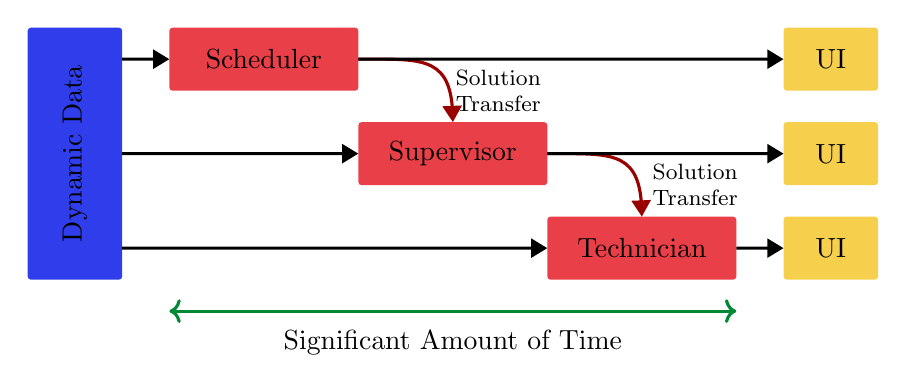
\begin{tikzpicture}[line width=0.0\basisb]
    \draw (2.0\basisb,4.0\basisb) 
		node[rotate=90, minimum height=3\basisb,fill=dtu-blue,minimum width=8\basisb,rounded corners=0.1\basisb] 
			(Dynamic Data) {Dynamic Data};

    \draw (8.0\basisb,7.0\basisb) 
		node[minimum height=2\basisb,fill=dtu-red,minimum width=6\basisb,rounded corners=0.1\basisb] 
			(Scheduler) {Scheduler};
    \draw (14.0\basisb,4.0\basisb) 
		node[minimum height=2\basisb,fill=dtu-red,minimum width=6\basisb,rounded corners=0.1\basisb] 
			(Supervisor) {Supervisor};
    \draw (20.0\basisb,1.0\basisb) 
		node[minimum height=2\basisb,fill=dtu-red,minimum width=6\basisb,rounded corners=0.1\basisb] 
			(Technician) {Technician};

    \draw (26.0\basisb,7.0\basisb) 
		node[minimum height=2\basisb,fill=dtu-yellow,minimum width=3\basisb,rounded corners=0.1\basisb] 
			(UserInterface1) {UI};
    \draw (26.0\basisb,4.0\basisb) 
		node[minimum height=2\basisb,fill=dtu-yellow,minimum width=3\basisb,rounded corners=0.1\basisb] 
			(UserInterface2) {UI};
    \draw (26.0\basisb,1.0\basisb) 
		node[minimum height=2\basisb,fill=dtu-yellow,minimum width=3\basisb,rounded corners=0.1\basisb] 
			(UserInterface3) {UI};

	\draw[<->, line width=0.1\basisb,color=dtu-green] (5.0\basisb, -1\basisb) -- (23.0\basisb, -1\basisb);
	\draw (14.0\basisb, -2.0\basisb) node {Significant Amount of Time};

	\draw[->,>=Triangle, thick, line width=0.1\basisb, color=dtu-corporate-red] (Scheduler) to[out=0, in=90,looseness=1.5]  (Supervisor);
	\draw[->,>=Triangle, thick, line width=0.1\basisb, color=dtu-corporate-red] (Supervisor) to[out=0, in=90,looseness=1.5] (Technician);
	\draw[->,>=Triangle, thick, line width=0.1\basisb] (Dynamic Data.south) ++(0\basisb,3.0\basisb) to[out=0, in=180,looseness=1.0] (Scheduler);
	\draw[->,>=Triangle, thick, line width=0.1\basisb] (Dynamic Data.south) to[out=0, in=180,looseness=1.0] (Supervisor);
	\draw[->,>=Triangle, thick, line width=0.1\basisb] (Dynamic Data.south) ++(0\basisb,-3.0\basisb) to[out=0, in=180,looseness=1.0] (Technician.west);
	\draw[<-,>=Triangle, thick, line width=0.1\basisb] (UserInterface1) to[out=180, in=0,looseness=1.0] (Scheduler);
	\draw[<-,>=Triangle, thick, line width=0.1\basisb] (UserInterface2) to[out=180, in=0,looseness=1.0] (Supervisor);
	\draw[<-,>=Triangle, thick, line width=0.1\basisb] (UserInterface3) to[out=180, in=0,looseness=1.0] (Technician);
	% \draw[<->, thick, line width=0.1\basisb] (Scheduler) -- (UserInterface);
	\begin{scope}[shift={(7,0)}] % Adjust shift to position the legend
    % Legend box
    % Legend lines and text
	    \draw[thick, line width=0.1\basisb] (-1.5,2.4) node[right, font=\footnotesize, align=center] {Solution\\Transfer};
	    \draw[thick, line width=0.1\basisb] (1.0,1.2) node[right, font=\footnotesize, align=center] {Solution\\Transfer};
	\end{scope}
\end{tikzpicture}

	\caption{
		Illustrates the bottlenecks and communication challenges inherent in hierarchical models, where lower-level processes depend heavily on higher-level outputs.
	}
	\label{fig:model-setup:classic-hierarchical}
\end{figure}

This project takes the approach shown in figure~\ref{fig:asynchronous_model_setup}. 
Instead of running an optimization algorithm once and then providing a stakeholder with a single 
solution, each algorithm runs in perpetuity always optimizing against the latest available information. This means that each algorithm will
be able to optimize based on the solutions that the other meta-heuristics finds. Also, through UI components stakeholder can interact with the
optimization process that corresponds to his part of the larger maintenance scheduling process. 

\begin{figure}[H]
	\centering
	\usetikzlibrary{positioning}
% \usetikzlibrary{arrows.meta}
\usetikzlibrary{bending}
\usetikzlibrary{backgrounds}
\definecolor{red}{HTML}{8A3F3A}
\definecolor{yellow}{HTML}{E0BB3C}
\definecolor{blue}{HTML}{4569E0}
\definecolor{green}{HTML}{17E561}
\definecolor{other}{HTML}{6A939E}

% DTU Colors
\definecolor{dtu-corporate-red}{HTML}{990000}
\definecolor{dtu-white}{HTML}{ffffff}
\definecolor{dtu-black}{HTML}{000000}
\definecolor{dtu-blue}{HTML}{2F3EEA}
\definecolor{dtu-bright-green}{HTML}{1FD082}
\definecolor{dtu-navy-blue}{HTML}{030F4F}
\definecolor{dtu-yellow}{HTML}{F6D04D}
\definecolor{dtu-orange}{HTML}{FC7634}
\definecolor{dtu-pink}{HTML}{F7BBB1}
\definecolor{dtu-grey}{HTML}{DADADA}
\definecolor{dtu-red}{HTML}{E83F48}
\definecolor{dtu-green}{HTML}{008835}
\definecolor{dtu-purple}{HTML}{79238E}


\newlength{\basisc}
\setlength{\basisc}{0.5cm}

\centering
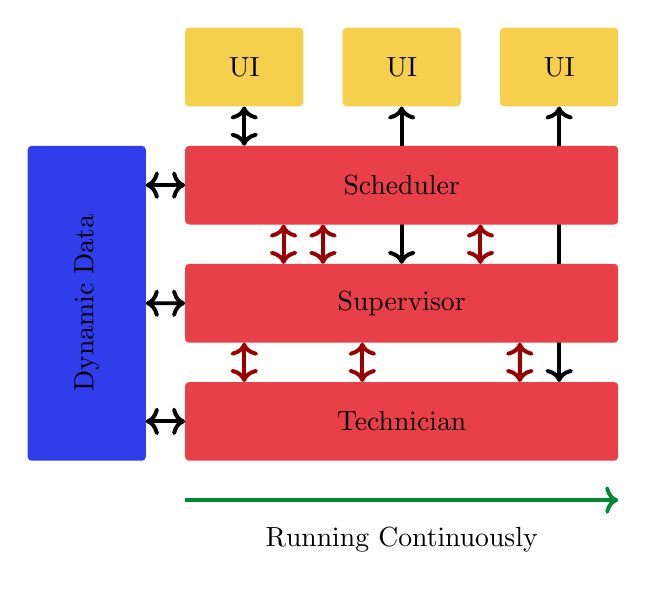
\begin{tikzpicture}[line width=0.0\basisc]
    \draw (4.0\basisc,4.0\basisc) 
		node[rotate=90, minimum height=3\basisc,fill=dtu-blue,minimum width=8\basisc,rounded corners=0.1\basisc] 
			(Dynamic Data) {Dynamic Data};

			

    \draw (8.0\basisc,10.0\basisc) 
		node[minimum height=2\basisc,fill=dtu-yellow,minimum width=3\basisc,rounded corners=0.1\basisc] 
			(UserInterface1) {UI};
    \draw (12.0\basisc,10.0\basisc) 
		node[minimum height=2\basisc,fill=dtu-yellow,minimum width=3\basisc,rounded corners=0.1\basisc] 
			(UserInterface2) {UI};
    \draw (16.0\basisc,10.0\basisc) 
		node[minimum height=2\basisc,fill=dtu-yellow,minimum width=3\basisc,rounded corners=0.1\basisc] 
			(UserInterface3) {UI};
    \draw (12.0\basisc,7.0\basisc) 
		node[minimum height=2\basisc,fill=dtu-red,minimum width=11\basisc,rounded corners=0.1\basisc] 
			(Scheduler) {Scheduler};
    \draw (12.0\basisc,4.0\basisc) 
		node[minimum height=2\basisc,fill=dtu-red,minimum width=11\basisc,rounded corners=0.1\basisc] 
			(Supervisor) {Supervisor};
    \draw (12.0\basisc,1.0\basisc) 
		node[minimum height=2\basisc,fill=dtu-red,minimum width=11\basisc,rounded corners=0.1\basisc] 
			(Technician) {Technician};


	\begin{pgfonlayer}{background}
		\draw[<->, thick, line width=0.1\basisc] (UserInterface1) to[out=-90, in=90,looseness=1.0] ++(0\basisc,-2.0\basisc)(Scheduler);
		\draw[<->, thick, line width=0.1\basisc] (UserInterface2) to[out=-90, in=90,looseness=1.0] (Supervisor);
		\draw[<->, thick, line width=0.1\basisc] (UserInterface3) to[out=-90, in=90,looseness=1.0] ++(0\basisc,-8.0\basisc)(Technician);

	\end{pgfonlayer}

	\draw[->, line width=0.1\basisc,color=dtu-green] (6.5\basisc, -1\basisc) -- (17.5\basisc, -1\basisc);
	\draw (12.0\basisc, -2.0\basisc) node {Running Continuously};

	\draw[<->, thick, line width=0.1\basisc, color=dtu-corporate-red] (Scheduler)++(-3\basisc, -1.0\basisc) to[out=-90, in=90,looseness=1.0]  ++(0\basisc, -1.0\basisc)(Supervisor);
	\draw[<->, thick, line width=0.1\basisc, color=dtu-corporate-red] (Scheduler)++(-2\basisc, -1.0\basisc) to[out=-90, in=90,looseness=1.0]  ++(0\basisc, -1.0\basisc)(Supervisor);
	\draw[<->, thick, line width=0.1\basisc, color=dtu-corporate-red] (Scheduler)++(2\basisc, -1.0\basisc) to[out=-90, in=90,looseness=1.0]  ++(0\basisc, -1.0\basisc)(Supervisor);

	\draw[<->, thick, line width=0.1\basisc, color=dtu-corporate-red] (Supervisor)++(-4\basisc, -1.0\basisc) to[out=-90, in=90,looseness=1.0] ++(0\basisc, -1.0\basisc)(Technician);
	\draw[<->, thick, line width=0.1\basisc, color=dtu-corporate-red] (Supervisor)++(-1\basisc, -1.0\basisc) to[out=-90, in=90,looseness=1.0] ++(0\basisc, -1.0\basisc)(Technician);
	\draw[<->, thick, line width=0.1\basisc, color=dtu-corporate-red] (Supervisor)++(3\basisc, -1.0\basisc) to[out=-90, in=90,looseness=1.0] ++(0\basisc, -1.0\basisc)(Technician);

	\draw[<->, thick, line width=0.1\basisc] (Dynamic Data.south) ++(0\basisc,3.0\basisc) to[out=0, in=180,looseness=1.0] (Scheduler);
	\draw[<->, thick, line width=0.1\basisc] (Dynamic Data.south) to[out=0, in=180,looseness=1.0] (Supervisor);
	\draw[<->, thick, line width=0.1\basisc] (Dynamic Data.south) ++(0\basisc,-3.0\basisc) to[out=0, in=180,looseness=1.0] (Technician.west);

	% \draw[<->, thick, line width=0.1\basisc] (Scheduler) -- (UserInterface);
\end{tikzpicture}

	\caption{
		Having metaheuristics continually running and coordinating state you can make a setup that is more robust by dynamically accepting inputs from the relevant stakeholder.  
	}
	\label{
		fig:asynchronous_model_setup
	}
\end{figure}

\textbf{Key Lessons:}
\begin{itemize}
	\item Hierarchical appraochs are problematic in practice, as the knowledge and information required for a high-quality and functioning maintenance 
		  scheduling process are usually found "lower in the hierarchy" rather than at higher levels, as managers sometimes implicitly believe.
	% \item Limitations of Hierarchical Approaches: Hierarchical models often fail because critical operational knowledge resides at lower levels.
	\item Having metaheuristics continuously running computational overhead as you only need to reach initial convergence once. Making the 
	      user experience more responsive and consecutive solutions will look more similar.
	\item Designing continuously running metaheuristics means that you have to think carefully about software architecture. Everything has to
		  be scalable, responsive, and dynamic. 
\end{itemize}

